%%%%%%%%%%%%%%%%%%%%%%%%%%%%%%%%%%%%%%%%%%%%%%%%%%%%%%%%%%%%%%%%%%%%%%%%%%%
% filename    : sp.tex
% author      : 
%%%%%%%%%%%%%%%%%%%%%%%%%%%%%%%%%%%%%%%%%%%%%%%%%%%%%%%%%%%%%%%%%%%%%%%%%%%

% use ateneo de naga etd class (actually modified virginia tech's etd class)
\documentclass[oneside]{etd}

% use these packages
\usepackage{graphicx}
%\usepackage{latexsym}
%\usepackage{amssymb}
%\usepackage[lineno5,noindent]{lgrind}
%\usepackage{rotating}
%\usepackage{makeidx}
%\usepackage{stmaryrd}
\usepackage{float}
%\usepackage{subfigure}
\usepackage{cite}
%\usepackage{moreverb}
%\usepackage{pictexwd,dcpic}
\usepackage{url}
%\graphicspath{{figs/}{./}}

%\renewcommand{\floatpagefraction}{0.8}

\makeindex

%%%%%%%%%%%%%%%%%%%%%%%%%%%%%%%%%%%%%%%%%%%%%%%%%%%%%%%%%%%%%%%%%%%%%%%%%%%

\title{Machine Assisted Data Capturing Process}
\author{My Name}
\department{Computer Science}
\BSdegree
\field{}
\degreemonth{June 23}  % date of final defense
\degreeyear{2014}

\threestudents
{John Michael C. Mariquit}
{Redan Benedict S. Alcaide}
{Kier Sostenes N. Guevara}

\threestudentsheader
{Mariquit, Alcaide, Guevara}

\threedegrees
{Computer Science}
{Computer Science}
{Computer Science}


\advisor
{Allan A. Sioson, PhD}
\threemembers
{Joshua C. Martinez, MIT}
{Jenilyn L. Agapito}
{Rey Herman R. Vidallo, MCS}
\deanandchair
{Allan A. Sioson, PhD}
{Jenilyn L. Agapito, MS}

\keywords{web service, android}


\begin{document}

\maketitle
\makerecomm
\makeacceptance
\makedeclaration

\begin{abstract}

	Our thesis focuses on the theoretical design and potential implementation of a data capturing system to be utilized on journal documents. The system shall identify pertinent information from the manuscript in question through parsing, and collate the identified data to specified fields pertaining to the required data for ranking by the pre-existing system of the Philippine Journal Citation Index Database, or PJCID. This is to be done in such a way as to avoid erroneous overlap, repetition or omission of data which shall be caused by widely varying formats of journals and citations.

	The ranking system  utilized by the PJCID has been fully documented and proved. The problem of the system, however, lies in the data acquisition and entry done for every new journal published. The data entry for the journal ranking system requires the users to manually encode every citation for every journal entry. The sheer amount of citations makes it tedious, time-consuming, and has the potentiality for errors and overlap.

	Our thesis aims to develop a system that is able to extract journal author information from documents of journal bibliographies and citations by parsing, then collate and relate the gathered information in such a way as to remove erroneous entries of journal information due to usage of varied citation formats. The system input shall rely upon documents from the users, which will be then parsed to extract relevant information.  The system output shall be a fully organized data of citations per entry, with accompanying data on authors, title and associated information. Any errors and its potential rate of generation found in the output of the system shall be studied in order to find the feasibility of the system.
\end{abstract}

\begin{dedication}

I dedicate this research work to all of humanity.

\end{dedication}


\begin{acknowledgements}

I thank everyone who helped me finish this thesis.

\end{acknowledgements}


\begingroup
\renewcommand*{\addvspace}[1]{}
\tableofcontents
\listoffigures
\listoftables
\endgroup

\beginbody
\pagenumbering{arabic}

%%%%%%%%%%%%%%%%%%%%%%%%%%%%%%%%%%%%%%%%%%%%%%%%%%%%%%%%%%%%%%%%%%%%%%%%%%%
\chapter{Introduction}
%%%%%%%%%%%%%%%%%%%%%%%%%%%%%%%%%%%%%%%%%%%%%%%%%%%%%%%%%%%%%%%%%%%%%%%%%%%
Journals publications, their entries and the authors of these entries, serve as one of important foundations of modern academic studies, serving as a convenient source of new discoveries and citation sources. However, finding the best of or even the reputable authors among the mass of entries and journals can be difficult to any reader. 

The primary method used by the community on ranking journal articles is through the amount of citations it has received from other articles. Citations also serve as auxiliary support for informational purposes, like indexing and ranking \cite{rank}, and quality assessment \cite{quality}. 

However, the flexibility of the citation system used by article authors give references of supposedly standardized citations massive potentiality for variation. This is the reason for the several journal citation index databases that has been implemented in many academic circles, a close example of which is the Philippine Journal Citation Index Database. Authors of studies, texts and documents published in the many academic journals around the world are ranked in these databases, giving users quick access to authors whose works have been referenced and trusted by many other authors to their own published papers.
\section{Project Context}
The Philippine Journal Citation Index Database, or PJCID, is a web-based citation index database funded by the Commission on Higher Education (CHED), Republic of the Philippines, in cooperation with Ateneo de Naga University, to track publications of Philippine Journals accredited by the Journal Accreditation Service (JAS) of CHED. The database currently has records of up to 44 Philippine-based journals, more than 1000 articles in total \cite{pjcid}.

The PJCID system records data on journal citations and all its associated information, like article authors and co-authors, article title, journals, publishers, along with year of publication and even kind of citations. The data collected will then be processed and resulting conclusions shall be displayed on the PJCID website as reports pertaining to the author, publisher or journal in question. The PJCID only focuses on direct citations -   articles citing earlier documents - and not bibliographic coupling - two or more articles sharing one or more references. \cite{citation}  
Data gathering for the PJCID system is relies on the manual input of data from the PJCID administrative team. Identification of necessary information from the myriad citation formats and forms is done by the people involved, and they will be the ones to input the identified data into the database. Properly identifying the information, however, has proven to be rife with difficulties, like unclear nomenclature, synonyms, and publication volume, which has been recorded with a yearly increase of 3.7%. \cite{probs}

In practice, searching articles for necessary information starts with title and author acquisition and continues with extraction of authors, titles, publishers and journals of entries of the reference section of the article. In reality, however, even advanced solutions for identifying related literature, like co-word analysis, collaborative filtering, Subject-Action-Object (SAO) structures or citation analysis do often not deliver satisfying results. \cite{sols} 

This forces the current implementation of the PJCID data acquisition process to a manual approach. This makes data acquisition time-consuming and tedious to the people involved, especially on journal articles with substantial citations used. This thesis aims to create a machine-assisted process for the data acquisition of PJCID, specifically the utilization of an automated parsing system for the extraction of necessary information from journal articles.

\section{Purpose and Description}
The purpose of this thesis is the creation of a machine-assisted process for the data acquisition of PJCID. It shall focus on the parsing of journal articles derived from PDF format documents of several Philippine-based journals, deriving information necessary for report and data generation within the PJCID ranking system, like authors, titles, and citations used, along with information regarding said citations. It is to be noted that the users themselves shall input the text taken from the available PDF documentation of the articles into the system to be developed.
This information shall be extracted from the input text by way of parsing, primarily using general citation formats commonly used by the many academic journals and certain keywords, an example of which is journal names, common among citations. 

The thesis shall also study any errors generated by the machine-assisted process, and compare its rate to that of the existing manual data acquisition process of the PJCID. A comparative study on the potential error rate for the machine-assisted process will serve as evidence for the potential feasibility of machine-assisted data acquisition process.

Implementation of the process in question shall be performed by way of a citation parser to be designed and implemented by the proponents. With the main difficulty of data acquisition from citations coming from the varied and uncommon nomenclature, particular focus for the design will be on coverage of as much potential variations of citation formats as possible. This includes, but is not limited to, lack of authors, shortened names, interchange of article title and journal name, lack of date, or lack of either journal or publisher name.

\section{Objectives}
The objective of this thesis is the development of a machine-assisted data acquisition process to be utilized specifically by the PJCID system. This end objective is further expounded by the following:
\begin{itemize}
	\item To study the various formats used by journal publications, both on articles and on citations
	\item To study and formulate possible variations of the aforementioned formats, and the particular formats and identifying characteristics of such variations;
	\item To create a front-end input system where users may input texts of information required taken from journal PDFs;
	\item To design and create a back-end parser that can extract the necessary data from articles, utilizing the plans and formats studied;
	\item To identify erroneous data from the parsed input, and remove said errors if possible;
	\item To categorize the parsed input to the information category used by the PJCID;
	\item To create an output file based on the above that shall be compatible to the PJCID system;
	\item To create a back-end system that shall upload the output into the PJCID system;
	\item To study any errors that could not be removed from the citation parser, and compare it to error rates of the existing acquisition process:
\end{itemize}
%\vfill\eject
\section{Scope and Limitations}
The thesis shall only focus on the data acquisition process of the Philippine Journal Citation Index Database. Thusly, the parsing system to be designed and implemented by the proponents shall be designed with the PJCID system in mind only. The citation parser to be designed and implemented by the proponents shall only focus on the information necessary for ranking. Journals to be used as test inputs will be ones based within the Philippines. These journals shall be in PDF format, with text transfer to the system to be done by the users themselves. The comparison of error rates shall be between the designed citation parser and the existing manual data acquisition process.

The system designed shall in no way focus on the process of ranking and display of information to the PJCID website, nor will it perform image-processing functions for PDF journal data extraction. The system shall only take in textual input taken by the users from PDF documentation, and add the processed data into the PJCID database. 
%%%%%%%%%%%%%%%%%%%%%%%%%%%%%%%%%%%%%%%%%%%%%%%%%%%%%%%%%%%%%%%%%%%%%%%%%%%
\chapter{Review of Related Systems and Related Literature}
%%%%%%%%%%%%%%%%%%%%%%%%%%%%%%%%%%%%%%%%%%%%%%%%%%%%%%%%%%%%%%%%%%%%%%%%%%%
	Journal ranking is used to evaluate the scientific impact of an academic paper in its respective area of research. Also, journal ranking may also be used to approximate the quality of an academic paper. An author's published work's relevance can be quantified by its citation impact.

	However, the ranking of authors, journals and publishers in the world of academic publication has far more impact than the creation of a list of article creators that are trusted by the academic community. These rankings can also have a substantial effect on the standing of those involved, giving greater credence to notable authors, popularity to successful journals and prestige to publishers with widely used articles. 

	This makes an improperly ranked journal listing dangerous, not only to the users, but to those listed as well. Thusly, ranking of articles and their proponents by way of citation has had many studies and modifications upon the processes utilized.

\section{Eigenfactor and Impact Factor}
In measuring citation impact, different measures may be employed although a naive way to do this is through its citation count \cite{citation_frequency}. The citation count is a simple frequency distribution of academic papers referencing another academic paper. Other metrics such as h-index and Eigenfactor may also be used in measuring citation impact.

H-Index is defined by Hirsch as "A scientist has index H if H of his or her Np papers have at least H citations each and the other (Np -– H) papers have ≤ H citations each" \cite{h_index}. To illustrate this, if an author X has an H-index of 25, this would mean that the author has 20 papers which have been cited 25 or more times. Then it can be said that the H-index is a measure of an author's productivity in relation to the number of papers published and how often his/her works are cited. To note, the H-index can only be applied to authors working in similar fields because conventions of citation vary among different fields.

The Eigenfactor is an algorithm used to rank journals based on cross-citation data \cite{eigenfactor_metrics}. Similar to how Google ranks its web pages via systems of hyperlinks, the Eigenfactor does so using the principle of Eigenvector centrality. First a "Citation Network" is built then the connections between citations are modeled. The importance of a journal is then ranked depending on its "centrality", which is determined by a journal's location in the network. The more citations a journal has, it can then be said that it is more "central" \cite{eigenfactor_rank}. Jevin D. West the original creator of the Eigenfactor algorithm, presented a modified version of the Eigenfactor which caters to author-level ranking by working on an author-level cross-citation matrix \cite{eigenfactor_influence}.

\section{Identity Uncertainty}

Identity uncertainty is a prevalent and unavoidable problem in citation matching. This phenomenon occurs if identifiers are absent in token sequences which may result in ambiguous observations for certain objects. This problem is addressed by constructing Relational Probability Models (RPMs) which consist of attributes that a citation may contain. RPMs semantics assume that unique names exist for different papers (although they may be the same) unless proven otherwise. Uniqueness is decided by the mapping which has the least co-referring terms. The RPMs can then be expressed to an equivalent Bayesian network where attributes of the objects are constructed as nodes. If citation C1 and C2 correspond to the paper P1 and P2 where P1 and P2 are the same object, the models will share one set of the same attributes \cite{identity_uncert}. A Markov Chain Monte Carlo based algorithm is then used to match the citations. \cite{markov}

\begin{figure}[H]
    \centering
    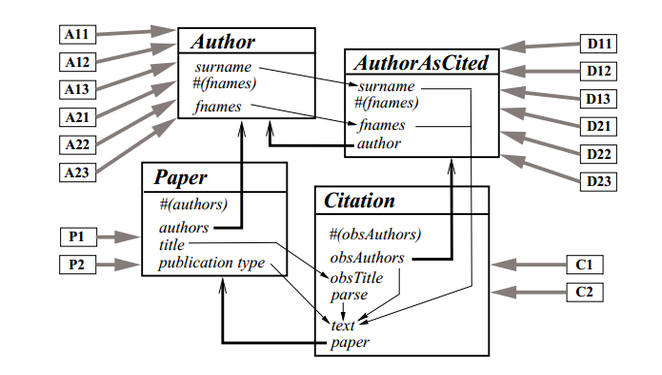
\includegraphics[width=0.8\textwidth]{RPM.png}
    \caption{Relational Probability Model}
    \label{fig:RPM}
\end{figure}

The image above serves as an example of our Citeseer. The large rectangles represent classes: the dark arrows indicate the ranges of their complex attributes, and the light arrows lay out all the probabilistic dependencies of their basic attributes. The small rectangles represent instances, linked to their classes with thick grey arrows. We omit the instance statements which set many of the complex attributes.

\section{Data Catching and Citation Parsing}

	In order to extract the necessary information, a parser is required to sift through the text and separate the necessary from the unnecessary. The problem of citation extraction is the segmentation of oftentimes unstructured or ill-structured citations into proper segments, where data and its classification can be properly identified. Several methods have been proposed in the recent years for the extraction of data from textual documents. The methods can be generally defined into two categories: knowledge-based approach, and learning -based approach. \cite{bibpro}

	The knowledge-based approach derives ontology that describes the data of interest using domain knowledge, where the knowledge includes relationships, lexical appearances and context keywords. From the parsing the ontology, several rules and an extractor can be generated, which is then used to extract the data. This particular method is more widely used in real-world applications, with a well-known example on CiteSeer. CiteSeer is a popular search engine and digital library that extracts metadata from citations using heuristics, with an identification accuracy of titles and authors at 80\% and page number accuracy of 40\% \cite{citeseer}.  However, the database that CiteSeer’s system relies on must be maintained by a domain expert, making the presence of such an expert necessary.

	Other applications of knowledge-based approach are CRAM \cite{cram}, FLUX-CiM \cite{flux}, and INFOMAP \cite{infmap}. CRAM develops an automatic segmentation system for its inputs by mining tables in relational databases and data warehouses. FLUX-CiM can automatically create ontology for a given area, constructed from an existing set of sample metadata records.  The FLUX-SiM dataset, its own set of reference data to be used for testing and benchmarking, contains citations from two domains, Computer Science and Health Science. INFOMAP relies on a tree-based representation scheme that organizes reference concepts in a hierarchical manner. For the six major citation formats, it has an overall average of 92.39\% \cite{bibpro}. The INFOMAP dataset has roughly 160,000 citations records in 6 different citation styles.

	The learning-based approach focuses on the classification of the citation data in question, using machine learning in order to solve it. This requires training data in order to function properly, slightly similar to the FLUX-CiM stated above. Currently, there are three major machine learning techniques, the Support Vector Machines \cite{svm}, Hidden Markov Model \cite{markov}, and Conditional Random Fields \cite{crf}.  They are used to extract information from research papers and journal articles, and has shown great performance to the Cora dataset. The Cora dataset is the most widely used benchmarking dataset for machine learning techniques \cite{cora}. 

This particular method has great adaptability, mainly due to its nature as a machine-learning method. However, it does possess some limitations. The quality of training data directly affects the performance of the method \cite{bibpro}. A faulty set of training data can render the entire process useless. 

	This machine-assisted process that this thesis will focus on shall be under knowledge-based approach. This method allows for the use of keywords and lexicons, without relying on the creation of proper training data. 

%%%%%%%%%%%%%%%%%%%%%%%%%%%%%%%%%%%%%%%%%%%%%%%%%%%%%%%%%%%%%%%%%%%%%%%%%%%
\chapter{Technical Background}
%%%%%%%%%%%%%%%%%%%%%%%%%%%%%%%%%%%%%%%%%%%%%%%%%%%%%%%%%%%%%%%%%%%%%%%%%%%

Blah, blah, and blah.

%%%%%%%%%%%%%%%%%%%%%%%%%%%%%%%%%%%%%%%%%%%%%%%%%%%%%%%%%%%%%%%%%%%%%%%%%%%
\chapter{Methodology}
%%%%%%%%%%%%%%%%%%%%%%%%%%%%%%%%%%%%%%%%%%%%%%%%%%%%%%%%%%%%%%%%%%%%%%%%%%%

Methodology stuff will appear here.


\section{Systems Analysis}

\section{Systems Design}

\section{Requirements Specification}

\section{Development and Testing}

%%%%%%%%%%%%%%%%%%%%%%%%%%%%%%%%%%%%%%%%%%%%%%%%%%%%%%%%%%%%%%%%%%%%%%%%%%%
\chapter{Contributions and Recommendations}
%%%%%%%%%%%%%%%%%%%%%%%%%%%%%%%%%%%%%%%%%%%%%%%%%%%%%%%%%%%%%%%%%%%%%%%%%%%

\section{Summary of Contributions}

Blah, blah, and blah.

\section{Implementation Plan}

Implementation plan in terms of Infrastructure and Deployment.




\appendix
\chapter{Code Listing}

The following is a source code listing of programs
developed in this research project.

\chapter{Evaluation Tool}

Evaluation tool used goes here.

\chapter{Sample Input/Output}

Describe and discuss the details of sample I/O here.

\chapter{Sample Reports}

Describe and discuss the details of sample reports here.

\chapter{User's Guide}




\nocite{*}
\bibliographystyle{siam}
{
\singlespace
\bibliography{sp}
}

\begin{vita}
JR is BS Information Technology student of the
Department of Computer Science at the Ateneo de Naga University.
\end{vita}



\end{document}
